\documentclass{article}

\usepackage[T1]{fontenc}
\usepackage{graphicx}
\usepackage{fancyhdr}
\pagestyle{fancy}
\fancyhf{}
\lhead{Version 1.4.1}
\rhead{Elliot Oram}
\rfoot{\thepage}


\title{Video Processor Class Diagram}
\author{elo9@aber.ac.uk}

\begin{document}

\maketitle
\tableofcontents

\newpage

\section{Video Processor Class Diagram}
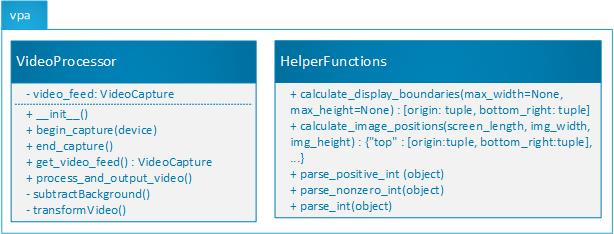
\includegraphics[width=\textwidth]{VideoProcessorClassDiagramImage}


\section{Description of Class Diagram}
The vpa (Video Processor Application) package contains two modules. The first, the \textbf{VideoProcessor} module, contains the \textbf{VideoProcessor} class which is the core of the system that will handle video capture and display. The second module will contain helper functions for the \textbf{VideoProcessor} class that do not require access to the class variables.

\subsection{VideoProcessor}
\subsubsection{Variables}
\begin{itemize}

	\item \textbf{video\_feed}: The video\_feed variable is of type VideoCapture. This class type holds a video stream and can be imported from OpenCV. To maximise the performance of the system the video object will be a global to the class object to avoid passing into and out of functions. However for test access there will be a get method for the video\_feed.

	\item \textbf{screen\_width}: variable of type int and stores the physical width of the screen (not resolution).
	
	\item \textbf{screen\_height}: variable of type int and stores the physical height of the screen (not resolution).
\end{itemize}

\subsubsection{Functions}

\begin{itemize}
	\item \textbf{\_\_init\_\_}: Python constructor for initialising the video\_feed object to None. Constructor also takes optional screen\_width and screen\_height for the physical screen dimensions. If these parameters are not given then the screen resolution will be used.
	
	\item \textbf{begin\_capture}: Function to start the video\_feed with specified device. This function takes an integer (referring to the device number to use - 0 is default) and sets the video\_feed to capture the video from that device. The function has a check to ensure that the parameter is an integer and raises a ValueError is it is not.
	
	\item \textbf{end\_capture}: Function to release the camera feed handle and set the video\_feed variable to None.
	
	\item \textbf{scale\_video\_feed}: This function will scale the video\_feed variable to the most ideal resolution. The most ideal resolution is calculated by the get\_ideal\_image\_resolution function. 
	
	\item \textbf{process\_and\_output\_video}: The output\_video function will add  4 copies of the video\_feed to a window in the correct locations. This function will also handle calls to subtract\_background and rotate\_image.
	
	\item \textbf{get\_video\_feed}: returns the video\_feed object.   

	\item \textbf{subtractBackground}: The subtractBackground function will be used to ensure that only the Actor is shown in the video feed and the background is removed (set to black (RGB(0,0,0)). Based on research stated in the Outline Project Specification, This will use simple background subtraction or moving average background subtraction. Spike solutions will be carried out during the creation of the prototype to assess if the image processing machine is capable of more complex background subtraction techniques. Furthermore, it will test if simple background subtraction techniques produce the required effect.

\end{itemize}


\subsection{HelperFunctions}
\subsubsection{Functions}

\begin{itemize}
	\item \textbf{get\_screen\_resolution}: Function that returns the screen resolution of the main monitor which the application is running on.

	\item \textbf{calc\_display\_area\_props}: This function take the specified maximum width and height of the display area and creates the largest possible square that will fit. The function then returns the length of a side of this square display area and the displacement of this display area from the corner of the screen. This function makes the assumption that the screen is wider than it is tall.
	
	\item \textbf{calculate\_image\_positions}: Calculates the co\-ordinates that each image (video frame) should be placed in. The images should be in the top\-middle, bottom\-middle, left\-middle and right\-middle of the screen. The screen length (one require one value for this as the display area is square), image width and image height are parameters of the function. The function will calculate to co-ordinates by finding using half the screen length + or - half the height or width of the image. The function will return a map of lists of tuples containing the co-ordinates. The map will be structured such that: \\
	\{"position" : [origin tuple, bottom right tuple],\\... \} \\
	An example of this is: \\
	\{"top" : [(100,0), (200,50)],\\... \}	
	
	\item \textbf{get\_ideal\_image\_resolution}: Given the length of one side of the square display area, this functions determines the maximum resolution an image should be. Images will be squares and can, at a maximum, be a third of the length of a side of the display area. This function will traverse a list of possible video resolutions and return that resolution as a tuple.
	
	\item \textbf{calculate\_crop\_range}: This function calculates the range to crop to image, post scale, to ensure it fits correctly in the display area. Given the resolution and maximum allowed image size, the function returns a list of the values to crop by in the form: [height\_start, height\_end, width\_start, width\_end].
	
	\item \textbf{rotate\_image\_anticlockwise}: Function that rotates an image (frame of the video - numpy array representation) anticlockwise. The function take the maximum image size and the rotation desired for the image in degrees. The function returns a numpy array that represents the image. 

\end{itemize}

\subsection{Parsers}
\subsubsection{Functions}
\begin{itemize}
	\item \textbf{parse\_int}: Takes an object, python variable, and raises an error if it is not a integer. 	
	
	\item \textbf{parse\_positive\_int}: Takes an object, python variable, and raises an error if it is not a positive integer

	\item \textbf{parse\_nonzero\_int}: Takes an object, python variable, and raises an error if it a zero.
	
\end{itemize}


\end{document}